\documentclass[a4paper,10pt]{article}
\usepackage{graphicx}

\usepackage[utf8]{inputenc}
\usepackage[portuguese,brazil]{babel}
\usepackage[T1]{fontenc}

\usepackage{algorithm}
\usepackage[noend]{algorithmic}
\usepackage{amsmath}

\usepackage{indentfirst}
\usepackage{url}

\usepackage{float}
\floatstyle{boxed}
\restylefloat{figure}

\renewcommand{\algorithmicrequire}{\textbf{Exija:}}
\renewcommand{\algorithmicensure}{\textbf{Garanta:}}
\renewcommand{\algorithmicend}{\textbf{fim}}
\renewcommand{\algorithmicif}{\textbf{Se}}
\renewcommand{\algorithmicthen}{\textbf{então}}
\renewcommand{\algorithmicelse}{\textbf{Senão}}
\renewcommand{\algorithmicelsif}{\algorithmicelse \textbf{, se}}
\renewcommand{\algorithmicendif}{\algorithmicend\ \algorithmicif}
\renewcommand{\algorithmicfor}{\textbf{Para}}
\renewcommand{\algorithmicforall}{\textbf{Para todo}}
\renewcommand{\algorithmicdo}{\textbf{faça}}
\renewcommand{\algorithmicendfor}{\algorithmicend\ \algorithmicfor}
\renewcommand{\algorithmicwhile}{\textbf{Enquanto}}
\renewcommand{\algorithmicendwhile}{\algorithmicend\ \algorithmicwhile}
\renewcommand{\algorithmicloop}{\textbf{Loop}}
\renewcommand{\algorithmicendloop}{\algorithmicend\ \algorithmicloop}
\renewcommand{\algorithmicrepeat}{\textbf{Repita}}
\renewcommand{\algorithmicuntil}{\textbf{até}}
\renewcommand{\algorithmicprint}{\textbf{Imprima}}
\renewcommand{\algorithmicreturn}{\textbf{Retorne}}
\renewcommand{\algorithmictrue}{\textbf{Verdadeiro}}
\renewcommand{\algorithmicfalse}{\textbf{Falso}}
\renewcommand{\algorithmiccomment}[1]{\hspace*{2em}// \textit{#1}}
\floatname{algorithm}{Algoritmo}

\begin{document}


\begin{titlepage}

\begin{minipage}{0.2\linewidth}
 
\includegraphics[]{./minerva.png}
\end{minipage}
\begin{minipage}{0.8\linewidth}
 \textbf{Universidade Federal do Rio de Janeiro}\\
 Instituto de Matemática\\
 Departamento de Ciência da Computação\\
 \rule{0.8\linewidth}{0.5mm}\\
 Rio de Janeiro, RJ - Brasil
\end{minipage}

\begin{center}

\vspace{2cm}

\Large
Trabalho de Simulação: Implementação e análise de um simulador.

\vspace{1cm}

\large

Gabriel Pires da Silva

\vspace{0.5cm}

Igor da Fonseca Ramos

\vspace{0.5cm}

Renan da Costa Garrot

\vspace{2.5cm}

\today

\normalsize
\end{center}

\vfill

\begin{flushright}
\begin{tabular}{rl}
Disciplina: & Avaliação e Desempenho 2011/2\\
Professores: & Daniel Sadoc Menasché\\
 & Paulo Henrique de Aguiar Rodrigues\\
\end{tabular}
\end{flushright}

\vspace{2cm}

\end{titlepage}

\pagebreak

\tableofcontents
\pagebreak

\listoffigures
\pagebreak

\section{Introdução}

A tarefa que nos foi atribuída consistia em implementar um simulador de um sistema \textit{peer-to-peer} com o objetivo de comparar os cenários apresentados e de acrescentar nossas observações sobre a escalabilidade dos mesmos.

A modelagem foi dada na descrição do trabalho e trata-se de uma simplificação de um sistema real. Estão presentes na simulação o \textit{publisher}, o qual é responsável por enviar o arquivo; os \textit{peers}, que desejam efetuar o download; e os \textit{seeds}, que são usuários comuns que já receberam todos os dados, mas continuam presentes para ajudar na distribuição. 

Ao longo da implementação, enfrentamos algumas dificuldades, mas cremos que o resultado final foi satisfatório. Este relatório tem por finalidade apresentar uma breve descrição do simulador implementado, a teoria por trás do que foi executado e os resultados finais obtidos.

\pagebreak

\section{Implementação do Simulador}

\subsection{Linguagem de programação e plataforma}

O simulador foi implementado na linguagem C++. Esta escolha foi baseada em três fatores. O primeiro diz respeito à eficiência, pois o programa faz uso intenso da CPU e, portanto, uma linguagem compilada para \textit{assembly} torna a execução muito mais rápida. O segundo foi a possibilidade de se programar utilizando orientação a objetos, o que foi fundamental para a forma como o código foi dividido, facilitando o entendimento e simplificando a modelagem. Por último, temos a familiaridade dos três integrantes do grupo com a programação em C++, o que permitiu que todos estivessem engajados no trabalho desde seu princípio sem que fosse necessário despender tempo aprendendo uma nova linguagem.

O compilador utilizado foi o GCC 4.6, encontrado na maioria das distribuições mais atualizadas de Linux e de fácil acesso para download. A plataforma em que foram executados todos os testes foi o Ubuntu 11.10, embora o sistema possa ser compilado para qualquer sistema operacional para o qual haja uma versão do GCC.

\subsection{Funcionamento geral}

O simulador pode ser utilizado a partir do executável chamado ``\textit{sim}'', criado dentro da pasta \textit{bin} pelo \textit{Makefile}. Deve ser passado como parâmetro um arquivo de entrada contendo as informações sobre os cenários a serem simulados.

Alternativamente, pode-se usar o comando já preparado no \textit{Makefile} através da linha ``\textit{make run}''. Para isso, basta alterar o arquivo ``\textit{cenarios.txt}'', presente na pasta raiz do projeto, incluindo ou removendo configurações a serem testadas.

É possível, ainda, com o auxílio do programa ``\textit{gnuplot}'', gerar diversos gráficos, dentre os quais os que encontram-se neste relatório, através do comando ``\textit{make graph}''.

No modo verborrágico, são impressas informações extras sobre as variáveis da simulação no console. Para utilizá-lo, basta adicionar ``\textit{-v}'' após o nome do arquivo de entrada ou utilizar os comandos ``\textit{make vrun}'' e ``\textit{make vgraph}''.

Todos os dados resultantes das simulações podem ser encontrados no arquivo ``\textit{resultados.txt}'', na raiz do projeto, e no conteúdo da pasta \textit{log}.

\subsection{Modelagem do sistema}

A utilização da orientação a objetos teve como finalidade organizar o programa em classes que representassem entidades do simulador. Ao todo, foram criadas sete classes. São elas:

\begin{itemize}
	\item \textbf{evento:} Representa todos os tipos de acontecimento que podem ocorrer e é utilizada para formar a fila de eventos a serem tratados. Guardam o tempo em que acontecerão e o seu tipo.
	\item \textbf{eventoChegadaPeer:} Herda de evento e representa apenas uma chegada de peer. Não há nenhuma informação adicional com relação à classe pai evento, servindo apenas como especificação de tipo.
	\item \textbf{eventoSaidaSeed:} Herda de evento e representa apenas a saída de um seed. Guarda, além das informações presentes em evento, qual seed irá sair.
	\item \textbf{eventoTransmissão:} Herda de evento e representa apenas as transmissões. Além das informações presentes em evento, guarda quem irá tentar enviar um bloco.
	\item \textbf{pessoa:} Representa todos os tipos de pessoa que podem estar presentes no sistema. Guarda uma identificação, o tipo (\textit{publisher}, \textit{peer} ou \textit{seed}) e todas as informações sobre o estado dos blocos e a cor.
	\item \textbf{geradorAleatorio:} Responsável por gerar números pseudoaleatórios para serem usados na simulação. Pode gerar valores de uma distribuição uniforme ou de uma distribuição exponencial.
	\item \textbf{simulador:} Responsável por executar a simulação de fato. Cada instância é responsável por executar a simulação sobre um conjunto de parâmetros.
\end{itemize}

A coleta dos dados é feita na função principal do programa e em alguns trechos específicos da simulação.

\subsection{Fila de eventos}

Para a implementação da fila de eventos foi utilizada uma heap de mínimo. Com isso, obtemos tempo de inserção de um novo evento $O(log\,n)$ e tempo de consulta ao próximo evento $O(1)$.

\subsection{Geração de variáveis aleatórias}

São utilizadas variáveis aleatórias de distribuição uniforme e exponencial para a simulação. O gerador de variáveis aleatórias recebe uma semente ou utiliza o número 1 como padrão.

Quando é requisitado um número aleatório com distribuição de probabilidade uniforme, multiplica-se o último resultado dado por 1000003 e calcula-se o resultado módulo 1073741789 - que é um número primo. Este resíduo é retornado como um valor pseudoaleatório.

Caso se deseje obter um valor aleatório com distribuição de probabilidade exponencial de média $1 / \mu$, utiliza-se um número pseudoaleatório com distribuição de probabilidade uniforme e calcula-se a inversa da CDF da distribuição exponencial para este valor. O resultado da aplicação desta função é retornado como um valor pseudoaleatório.

\pagebreak

\section{Simulações}

\subsection{Variáveis observadas}

Foram observadas as seguintes variáveis aleatórias ao longo da simulação:
\begin{itemize}
	\item \textbf{\textit{T}} $\overset{\underset{\mathrm{\Delta}}{}}{=}$ Tempo de permanência de um indivíduo no sistema.
	\item \textbf{\textit{D}} $\overset{\underset{\mathrm{\Delta}}{}}{=}$ Tempo de download do arquivo.
	\item \textbf{\textit{V}} $\overset{\underset{\mathrm{\Delta}}{}}{=}$ Vazão do sistema.
	\item \textbf{\textit{N}} $\overset{\underset{\mathrm{\Delta}}{}}{=}$ Número de pessoas presentes no sistema em um dado momento.
	\item \textbf{\textit{P}} $\overset{\underset{\mathrm{\Delta}}{}}{=}$ Número de \textit{peers} presentes no sistema em um dado momento.
	\item \textbf{\textit{S}} $\overset{\underset{\mathrm{\Delta}}{}}{=}$ Número de \textit{seeds} presentes no sistema em um dado momento.
\end{itemize}

É possível observar que algumas das variáveis observadas são redundantes, pois podem ser obtidas a partir de outras. Podemos, por exemplo, obter a média de $T$ a partir da média de $N$ utilizando o resultado de Little. O principal motivo que nos levou a escolher monitorar todas estas variáveis, mesmo sem aparente necessidade, foi a ajuda que isso nos proporcionou nos testes de corretude, como deixaremos mais claro na seção \ref{TestesDeCorretude}.

\subsection{Método}

Para cada conjunto de parâmetros foi utilizada uma simulação diferente utilizando o método \textit{batch}, ou seja, execuções em sequência de modo que os indivíduos remanescentes de uma rodada servem como condição inicial para a rodada seguinte. Como é requisito deste método, a cada peer que chegava era atribuída uma cor de modo que era possível considerar seus dados apenas no momento adequado.

Caso, por exemplo, um indivíduo receba a cor vermelha correspondente à rodada 2 da simulação e sua saída ocorra ainda nesta rodada, seu tempo de permanência influenciará a média da variável $T$, seu tempo de download será icluído na média da variável $D$, sua presença contará para as médias de $N$, $P$ e $S$ e sua saída afetará a variável $V$.

Por outro lado, caso este mesmo indivíduo termine o download ainda na segunda rodada, mas permaneça como \textit{seed} posteriormente, seu tempo de permanência não será utilizado em nenhum cálculo. Da mesma forma, sua saída não alterará nehuma vazão, embora sua presença ainda influencie as váriáveis $N$ e $S$ das rodadas seguintes.

Ainda, se ele sequer terminar o download antes do fim da rodada 2, ele influenciará $N$, $P$ e $S$ das rodadas seguintes, mas seu tempo de download e seu tempo de permanência serão descartados. Sua saída também não será contada para nenhuma vazão.

\subsection{Fase transiente} %Detecção do fim, principalmente

A fase transiente é o período em que o sistema ainda não está em equilíbrio, de forma que os resultados obtidos ao longo dela não são confiáveis e tendem a aumentar a variância e, com isso, aumentar o intervalo de confiança. Nosso objetivo é, portanto, tentar encontrar o seu fim para que possamos desconsiderá-la em nossos resultados.

Determinar o final da fase transiente é uma tarefa que depende de heurísticas, ou seja, não há nenhum método que nos forneça um resultado exato. Tentamos, então, determinar uma heurística que nos desse uma boa aproximação e nossa opção foi dada pelo seguinte algoritmo:

\begin{algorithm}[H]
	\caption{Heurística para detecção do final da fase transiente}
	\label{algoritmoFaseTransiente}
	\begin{algorithmic}
		\STATE Faça $X0 = 0$
		\STATE Faça $\Delta = 500$
		\STATE Faça $k = 5000$
		\STATE Faça $p = 0,025$
		\STATE Seja $c$ o número de chegadas até o momento
		\FOR{cada chegada}
			\IF{$c < k$}
				\STATE Ignore
			\ELSIF{$c - k$ é múltiplo de $\Delta$}
				\STATE Seja $X1$ a média da variável $X$
				\IF{$X1 - X0 < p * X1$}
					\STATE Encerre a fase transiente
				\ELSE
					\STATE $X0 \leftarrow X1$
				\ENDIF
			\ENDIF
		\ENDFOR
	\end{algorithmic}
\end{algorithm}

Os valores de $c$, $k$ e $p$ foram determinados expermientalmente através de diversos testes. Optamos, no final, por aqueles que proporcionaram bons resultados sem estender demais a fase transiente, pois deixá-la muito longa significa aumentar o tempo de execução do programa sem a contrapartida de resultados melhores.

Podemos observar o comportamento de algumas variáveis através dos gráficos nas figuras \ref{grafTransienteCen4b02n12rf} e \ref{grafTransienteCen6b10n40rr}. Nestes casos o final da fase transiente foi detectado de maneira satisfatória.

Na figura \ref{grafTransienteCen4b02n12rf}, a fase transiente foi concluída com 13500 chegadas. Podemos observar que isto ocorre no momento aproximado em que as curvas que representam o número médio de \textit{peers} no sistema e a média da vazão tornam-se estáveis.

De forma semelhante, na figura \ref{grafTransienteCen6b10n40rr} temos os tempos de download e de permanência aproximando-se de uma estabilidade em um momento próximo das 11500 chegadas, quando a heurística determinou como final da fase transiente.

Apesar do sucesso nestes dois casos, podemos observar nas figuras \ref{grafTransienteCen5b10n43rr} e \ref{grafTransienteCen1lamb0.9} que houve algumas situações em que a fase transiente poderia ter sido estendida, pois ainda havia grande variação nas médias. Na primeira, o fim da fase transiente terminou, para o simulador, após 7500 chegadas e, na segunda, após 49500. Em ambos os casos, podemos notar que se tratava de um período de aparente estabilidade da média, seguido por novas variações acentuadas.

Mesmo com casos como os dois últimos, o resultado final não foi insatisfatório, como discutiremos na seção \ref{ColetaDosDados}, e tornar a heurística mais restritiva não apresentou melhora visível. Desta forma, optamos por fixar os valores de $k$, $c$ e $\Delta$ naqueles exibidos no algoritmo \ref{algoritmoFaseTransiente}.

\pagebreak

\begin{figure}
	\caption{Cenário 4 com 12 pessoas e política \textit{rarest piece first} para os blocos}
	\label{grafTransienteCen4b02n12rf}
	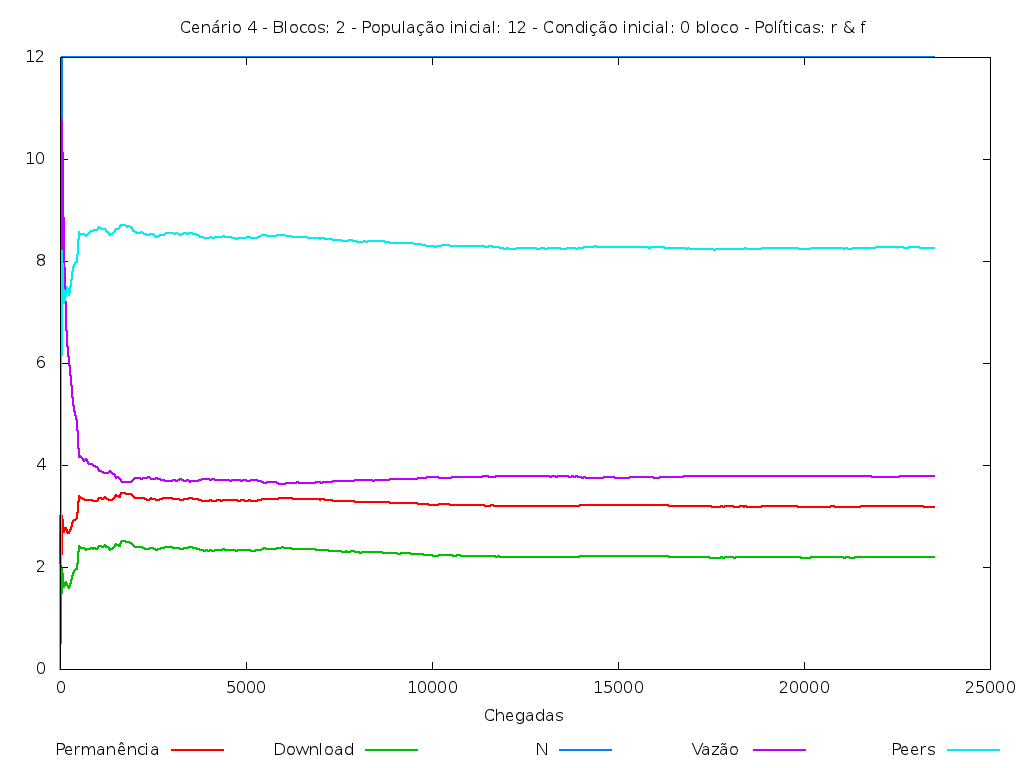
\includegraphics[scale = 0.33]{./graficos/faseTransiente/01.png}
\end{figure}

\begin{figure}
	\caption{Cenário 6 com 10 blocos e 40 pessoas}
	\label{grafTransienteCen6b10n40rr}
	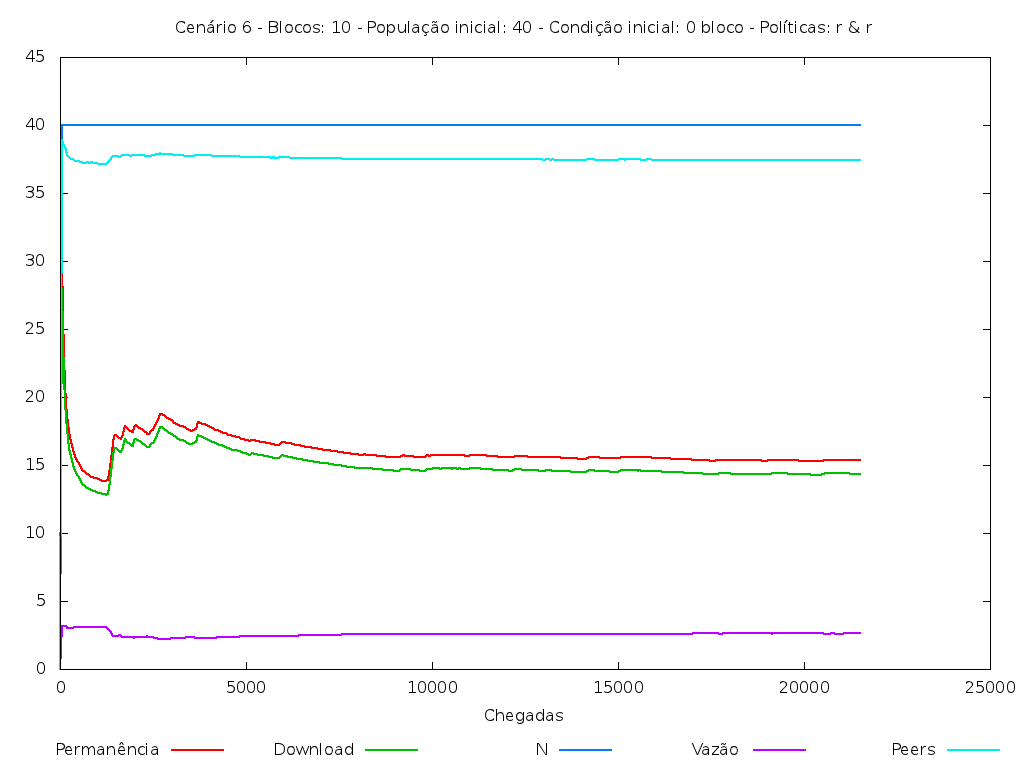
\includegraphics[scale = 0.33]{./graficos/faseTransiente/02.png}
\end{figure}

\clearpage

\begin{figure}
	\caption{Cenário 5 com 10 blocos e 43 pessoas}
	\label{grafTransienteCen5b10n43rr}
	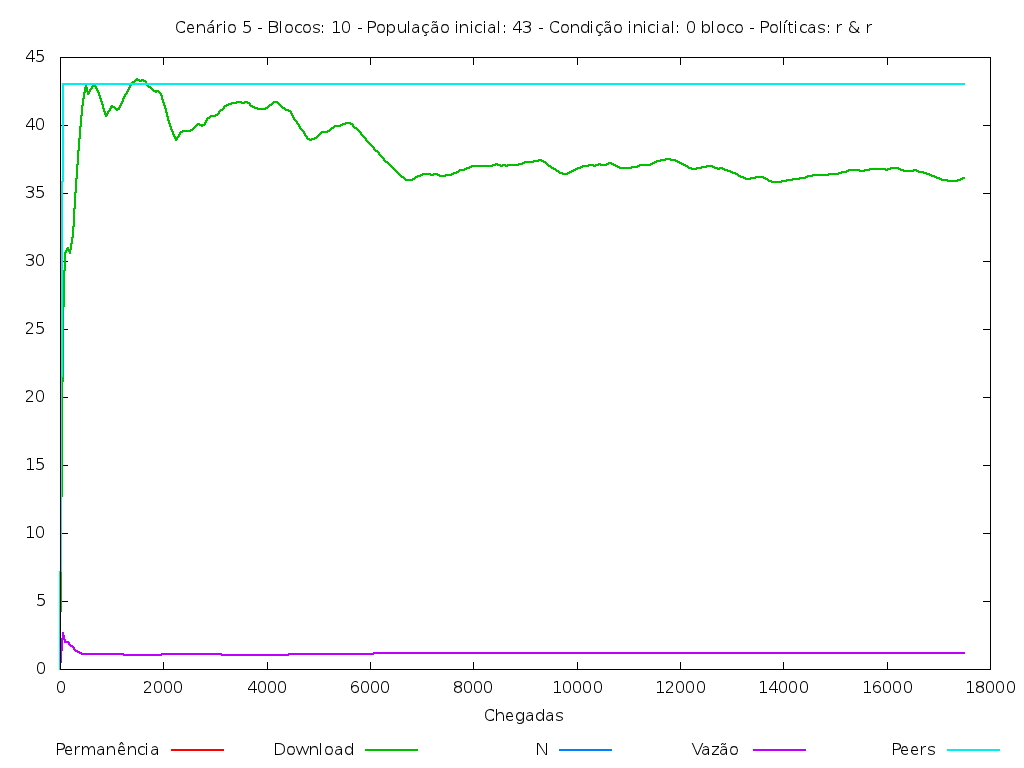
\includegraphics[scale = 0.33]{./graficos/faseTransiente/03.png}
\end{figure}

\begin{figure}
	\caption{Cenário 1 com $\lambda$ valendo 0,9}
	\label{grafTransienteCen1lamb0.9}
	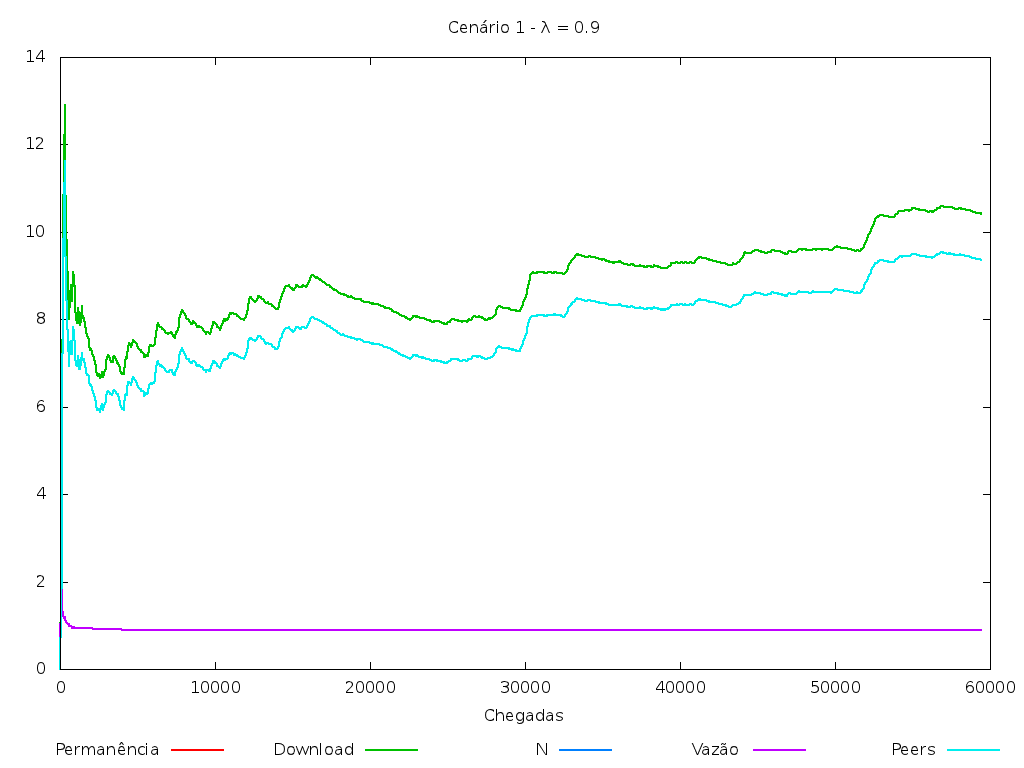
\includegraphics[scale = 0.33]{./graficos/faseTransiente/04.png}
\end{figure}

\clearpage
\pagebreak

\subsection{Rodadas}

Para que os intervalos de confiança sejam pequenos, é preciso que cada rodada tenha um bom tamanho e que o número total de rodadas seja suficientemente grande. Inicialmente, fixamos esses números em 30 rodadas com 5000 chegadas cada, mas alguns intervalos ainda estavam grandes demais e decidimos passar a 100 rodadas.

Posteriormente, aumentamos o tamanho de cada rodada para 10000 chegadas quando buscávamos o motivo de um determinado resultado não seguir padrão que esperávamos. Mesmo tendo resolvido esta questão de outra forma, optamos por manter, no final, um total de 100 rodadas com 10000 chegadas cada.

\pagebreak

\section{Testes de Corretude}\label{TestesDeCorretude}

Para testar nossa implementação, comparamos a saída do simulador com resultados que poderíamos obter analiticamente. Desta forma, fomos capazes de concluir quando o programa estava muito próximo de estar correto.

O cenário 1 proposto na descrição do trabalho representa exatamente uma M/M/1, visto que temos o arquivo com apenas um bloco, chegadas de peers seguindo um processo Poisson e a ausência total de seeds ou chegadas por recomendação. Dado que a disciplina de atendimento não afeta a média das variáveis observadas, podemos calcular analiticamente todos os resultados e compará-los com a saída da simulação. Com isso, pudemos executar o ajuste inicial do programa.

\subsection{Dificuldades enfrentadas}

Apesar de os testes com o cenário 1 terem eliminado a maior parte de nossas dúvidas, tivemos um grande problema já no final do desenvolvimento. Ao executar as simulações, percebemos que as vazões dos cenários 4 a 6 não se comportavam exatamente como esperado.

Esta falha nos tomou vários dias para ser resolvida. Uma das causas foi não sabermos como calcular analiticamente o resultado esperado para nos certificarmos de que, de fato, havia algo errado.

Outra causa foi o efeito do erro nos resultados. O problema no código fazia com que simplesmente simulássemos um cenário diferente daquele que esperávamos. Com isso, tínhamos o resultado de Little valendo para todas as variáveis e isso fez com que, novamente, ficássemos em dúvida se havia mesmo algum erro.

Terminamos por descobrir que, quando um peer chegava por recomendação, ele não transmitia nenhum dado. Desta forma, simulávamos um cenário em que um peer chegava, só recebia o arquivo do publisher e poderia ou não ficar um tempo no sistema sem fazer nada de fato. Uma vez corrigido o problema, obtivemos os dados apresentados nas próximas seções deste relatório.

\pagebreak

\section{Coleta dos dados}\label{ColetaDosDados}

\subsection{Cálculo de estimadores e intervalos de confiança} %Incremental

\subsection{Dados obtidos} %Apresentação dos requisitos do trabalho aqui

\pagebreak

\section{Interpretação dos resultados}

\pagebreak

\section{Conclusão}

\pagebreak

\section{Considerações finais}

\pagebreak

\end{document}


\begin{figure}
	\caption{Variância da V.A. $W_2$, Serviço LCFS com $\lambda$ = 0.40}
	\label{figTransienteLCFSfila2VarWLambda040}
	\includegraphics[scale = 0.20]{./graficos_transiente_2/08.png}
\end{figure}


\begin{centering}
\begin{table}[htp]
\makebox[\textwidth] 
{
\begin{tabular} { | c | c | c | c | c | r | }
    \hline
    Filas & $\lambda$  & Fase transiente  & Número de rodadas & Tamanho das rodadas  & FATOR \\ \hline
    FCFS     & $0.1$   & 10000 & 490     & 720      & 362800       \\ \hline
    FCFS     & $0.2$   & 10000 & 640     & 770      & 502800       \\ \hline
    FCFS     & $0.3$   & 10000 & 950     & 940      & 903000       \\ \hline
    FCFS     & $0.4$   & 10000 & 640     & 4100    & 2634000     \\ \hline
    FCFS     & $0.45$ & 50000 & 1110   & 8360    & 9329600     \\ \hline
    LCFS     & $0.1$   & 10000 & 320     & 1240    & 406800       \\ \hline
    LCFS     & $0.2$   & 10000 & 640     & 960      & 624400       \\ \hline
    LCFS     & $0.3$   & 10000 & 950     & 1260    & 1207000     \\ \hline
    LCFS     & $0.4$   & 10000 & 640     & 7300    & 4682000     \\ \hline
    LCFS     & $0.45$ & 50000 & 950     & 18700  & 17815000   \\ \hline
\end{tabular}
}
\caption{Fator Mínimo para cada simulação}
\label{TabelaFinal}
\end{table}
\end{centering}





\begin{figure}
	\caption{Variância da V.A. $W_2$, Serviço LCFS com $\lambda$ = 0.40}
	\label{figTransienteLCFSfila2VarWLambda040}
	\includegraphics[scale = 0.20]{./graficos_transiente_2/08.png}
\end{figure}